\documentclass{article}

\usepackage{amsmath, graphicx, amssymb, epigraph}

\title{Revis\~ao R\'apida de Processos At\^omicos e Nucleares}
\author{Rafael Lopes de S\'a}
\date{\today}

\begin{document}
\maketitle
\tableofcontents

\newpage

\section{Efeito fotoel\'etrico}

\epigraph{Ein Opfer an den physikaliscen Überzeugungen. Ein Akt der Verzweiflung.}{Max Planck}

O efeito fotoel\'etrico consiste num el\'etron de um metal absorvendo um f\'oton de forma que esse el\'etron se torna livre:

\begin{equation}
\text{el\'etron ligado} + \text{f\'oton} \rightarrow \text{el\'etron livre}
\end{equation}



Se a energia do f\'oton absorvida pelo el\'etron for maior que a energia de liga\c c\~ao do el\'etron com a estrutura met\'alica, o el\'etron vai se tornar livre e pode formar uma corrente el\'etrica. Quase todo problema sobre efeito fotoel\'etrico se resolve usando conserva\c c\~ao de energia. Conceitualmente:

\begin{equation}
\begin{split}
(\text{energia do f\'oton}) &- (\text{energia gasta para liberar o f\'oton da estrutura met\'alica}) = \\
&(\text{energia cin\'etica do el\'etron livre}) + (\text{energia potencial do el\'etron livre})
\end{split}
\end{equation}

A energia gasta para liberar o f\'oton da estrutura met\'alica \'e algo complicado de se calcular e, em geral, representamos apenas por um s\'imbolo $\phi$ e pelo nome ``fun\c c\~ao trabalho''. \'E uma propriedade do metal e n\~ao do f\'oton.

A energia de um f\'oton \'e proporcional \`a sua freq\"u\^encia:
\begin{equation}
E_f = hf,
\end{equation}
onde $h$ \'e chamado de \textbf{constante de Planck}. A energia cin\'etica \'e dada pela f\'ormula familiar:
\begin{equation}
E_c = \frac{1}{2}mv^2.
\end{equation}
J\'a a energia potencial depende do seu sistema. Usualmente uma bateria pode ser conectada \`a celula fotoel\'etrica criando uma diferen\c ca de potencial. O el\'etron tem que ent\~ao ir de contra (se o polo positivo da bateria estiver ligado ao cotodo) ou a favor (de o polo negativo da bateria estiver ligado ao catodo) esse potencial e gastar\'a ou, respectivamente, receber\'a uma energia dada por:
\begin{equation}
E_p = Q_e\times V,
\end{equation}
onde $Q_e$ \'e a carga do el\'etron e V \'e a diferen\c ca de potencial da bateria. Colocando todos os conceitos juntos:
\begin{equation}\label{eq:energia}
hf - \phi = E_c + E_p = \frac{1}{2}mv^2 + Q_eV.
\end{equation}

Algumas coisas a se lembrar:
\begin{itemize}
\item No efeito fotoel\'etrico usual, cada f\'oton \'e absrovido por um el\'etron. Isso quer dizer que se a energia do f\'oton n\~ao for pelo menos a fun\c c\~ao trabalho $\phi$, n\~ao haver\'a corrente el\'etrica. No caso em que h\'a uma bateria tamb\'em, a energia do f\'oton tem que ser, pelo menos, a fun\c c\~ao trabalho mais a energia potencial provida pela bateria.
\item Se o el\'etron absorver um f\'oton de energia maior (isto \'e, de maior frequ\^encia), ele sair\'a com maior energia. Mas \textbf{n\~ao quer dizer que mais el\'etrons ser\~ao emitidos}.
\item Para emitir mais el\'etron, voc\^e precisa de mais f\'otons. Isso quer dizer uma luz incidente mais intensa.
\end{itemize}

\subsection{Constantes e unidades}

A unidade de energia no Sistema Internacional de unidades \'e o Joule. $1\,\text{J}$ \'e uma quantidade muito grande para efeitos at\^omicos e subat\^omicos. Uma unidade conveniente \'e o $\text{eV}$. 1 $\text{eV}$ \'e definido como a energia que 1 (um) el\'etron tem num potencial de 1 (um) Volt. Para converter para o SI, basta usar a carga do el\'etron:

\begin{itemize}
\item $1\,\text{eV} = 1.6\times 10^{-19}\text{J}$,
\item $1\,\text{J} = 1/(1.6\times 10^{-19})\,\text{eV} = 6.24\times 10^{18}\,\text{eV}$ ,
\end{itemize}
pela pr\'opria defini\c c\~ao de $\text{eV}$ a carga el\'etrica fundamental \'e escrita como $e = 1.6\times 10^{-19}\,\text{C} = 1\,\text{eV/V}$.

Algumas constantes:

\begin{itemize}
\item $h = 6.626\times 10^{-34}\,\text{J s} = 4.136\times 10^{-15}\,\text{eV s}$,
\item $c = 3\times 10^{8}\,\text{m/s}$.
\item $hc = 1240\,\text{eV nm}$
\end{itemize}
O valor de $hc$ \'e conveniente porque, muitas vezes, \'e dado o comprimento de onda ($\lambda$) do f\'oton em vez da freq\"u\^encia. Essas duas quantidades se relacionam por:

\begin{equation}
c = \lambda f,
\end{equation}
logo, a energia de um f\'oton com comprimento de onda $\lambda$ \'e dada por:
\begin{equation}
E = hf = \frac{hc}{\lambda}.
\end{equation}

Algumas vezes tamb\'em \'e conveniente usar $\text{eV/c}^2$ como unidade de massa e $eV/c$ como unidade de momento linear. Nessa unidade, a massa do el\'etron é dada por:
\begin{equation}
m_e = 511\, \text{keV/c}^2.
\end{equation}

\subsection{Um exemplo t\'ipico}

A figura abaixo representa o arranjo t\'ipico do efeito fotoel\'etrico:

\begin{figure}[h]
\centering
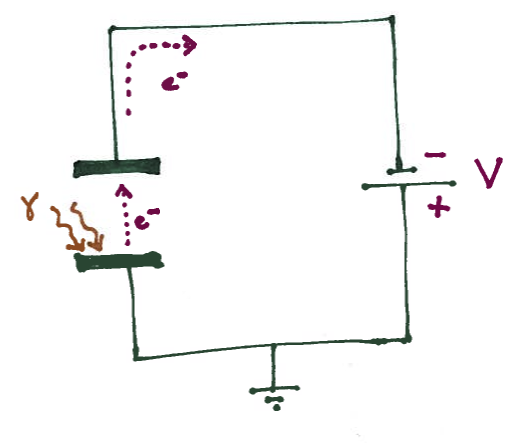
\includegraphics{circuito.png}
\caption{Arranjo t\'ipico do efeito fotoel\'etrico. Note que a luz indice sobre a placa inferior, chamada \textbf{anodo}, enquanto a placa superior, chamada \textbf{catodo}, coleta el\'etrons que conseguem se libertar do metal do anodo e est\~ao no v\'acuo entre as placas. Para mais detalhes veja texto.}
\end{figure}
A luz incide sobre a placa inferior. Se os f\'otons tiverem mais energia que a \textbf{fun\c c\~ao trabalho}, isto \'e, que a energia necess\'aria para liberar os el\'etrons da estrutura met\'alica, esse el\'etrons v\~ao escapar para o v\'acuo entre as placas, como representado pela seta pontilhada. Contudo, note que h\'a tamb\'em uma bateria no circuito. Essa bateria faz com que o fio na parte de cima esteja num potencial diferente do fio embaixo. Se assumirmos que o potencial do fio embaixo \'e 0, o potencial do fio de cima ser\'a negativo. Voc\^e pode dizer isso pela orienta\c c\~ao da baterial: veja que o terminal negativo (linha curta) est\'a ligada ao fio de cima.

Como el\'etrons s\~ao negativos e o potencial \'e negativo, os el\'etrons experimentam uma for\c ca contra seu movimento. Dito de outra forma, como tanta a carga do el\'etron quando o potencial el\'etrico \'e negativo, ent\~ao a energia potencial do fio em cima:

\begin{equation}
E_p = Q_E\times V > 0,
\end{equation}
\'e positiva. Num an\'alogo gravitacional, \'e como se houvesse uma montanha que os el\'etrons tem que subir e eles s\'o conseguem entrar no fio de cima se subirem essa montanha. Isto quer dizer que os el\'etrons tem que gastar essa energia potencial para conseguir se propagar no fio. Isso, claro, al\'em da energia gasta para se liberar da estrutura met\'alica (fun\c c\~ao trabalho). Desta forma, a energia cin\'etica do el\'etron \'e dada pela equ\c c\~ao~\eqref{eq:energia}:
\begin{equation}
E_c = hf - \phi - Q_e\times V.
\end{equation}
A energia cin\'ética \'e um n\'umero maior ou igual a zero. Quando a energia cin\'etica dos el\'etrons \'e zero, isso quer dizer que n\~ao h\'a corrente el\'etrica (os el\'etrons n\~ao chegam no catodo). O potencial para o qual isso acontece \'e dado por:
\begin{equation}
0 = hf - \phi - Q_e\times V_{\text{max}}.
\end{equation}
Essa \'e uma maneira muito conveniente de se medir a fun\c c\~ao trabalho de um potencial. Dado que voc\^e sabe a freq\"u\^encia do f\'oton e o potencial da baterial em que a corrente cessa ($V_{\text{max}}$), a fun\c c\~ao taabalho pode ser encontrada resolvendo a equa\c c\~ao acima:
\begin{equation}
\phi = hf - Q_e\times V_{\text{max}}.
\end{equation}

\subsection{Sobre a energia cin\'etica dos el\'etrons}
Para entender a energia cin\'etica que os el\'etrons ter\~ao no circuito \'e importante primeiro entender a energia que eles tem enquanto est\~ao num s\'olido. Isso pode ser visto no diagrama da figura \ref{fig:bandas}. Sem a incid\^encia de luz, os el\'etrons com maior energia num metal estar\~ao na banda intermedi\'aria. Essa \'e a chamada banda de condu\c c\~ao. Isso quer dizer que eles podem se propagar livremente dentro do material (por isso que metais conduzem eletricidade), mas n\~ao podem escapar do material. A energia de el\'etrons livre \'e maior que el\'etrons de condu\c c\~ao e a diferen\c ca entre as duas bandas de energia \'e justamente a fun\c c\~ao trabalho que j\'a definimos acima.

\begin{figure}[ht]
\centering
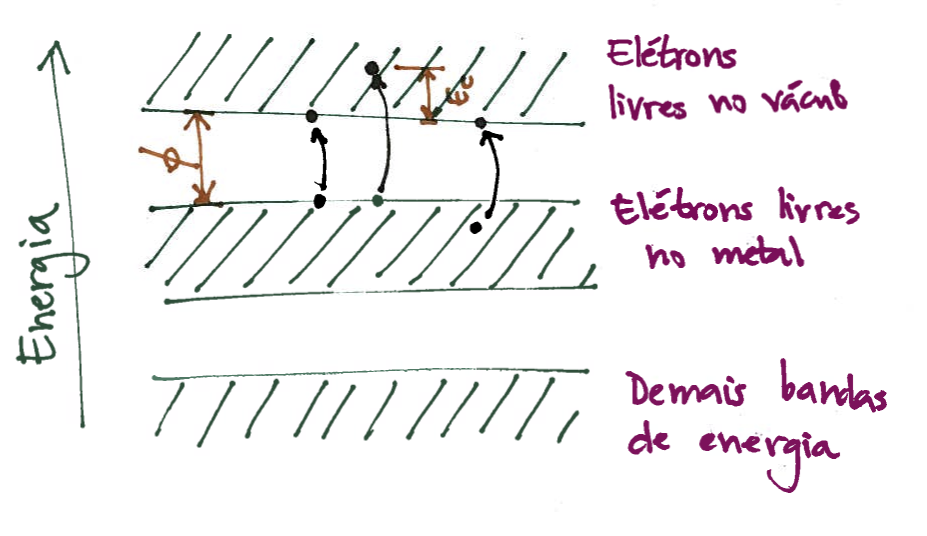
\includegraphics[width=0.9\textwidth]{bandas.png}
\caption{\label{fig:bandas}Estrutura de energia em bandas de um el\'etron num s\'olido. A figura mostra a chamada \textbf{banda de condu\c c\~ao}, na qual os el\'etrons podem se propagar livremente dentro do material e a diferen\c ca de energia $\phi$ para que os el\'etrons escapem do estrutura do material e possam se propagar livremente no v\'acuo fora do material. A diferen\c ca de energia entre essas duas bandas de energia \'e chamada \textbf{fun\c c\~ao trabalho} $\phi$.}
\end{figure}
Note que s\'olidos s\~ao essencialmente diferente de \'atomos livres. Em \'atomos livres (como num g\'as), os el\'etrons s\'o podem ter energias discretas bem definidas. Em s\'olidos eles podem ter \textbf{qualquer energia} em \textbf{bandas de energias}. Ent\~ao podemos imaginar diversas situa\c c\~oes distintas para como o efeito fotoel\'etrico ocorre no metal. Os tr\^es casos que quero discutir s\~ao representados pelas tr\^es setas escuras.

No primeiro caso (mais a esquerda), o el\'etron absorve um f\'oton que tem energia \textbf{exatamente} igual a fun\c c\~ao trabalho. Isso quer dizer que o el\'etron s\'o vai sair do material se ele tiver a maior energia poss\'ivel na banda de condu\c c\~ao. Se a energia dele fosse um poquinho menor, ele n\~ao escaparia. E, mesmo quando escapa, ele fica livre, mas parado, pois n\~ao sobra nenhuma energia como energia cin\'etica.

Nos dois outros casos o f\'oton tem mais energia que a fun\c c\~ao trabalho. Ent\~ao duas coisas podem acontecer. Esse f\'oton pode ser absorvido por um el\'etron na borda da banda de condu\c c\~ao, isto \'e, com a maior energia poss\'ivel dentro do material. Neste caso, o el\'etron se libera e ainda ter\'a uma energia cin\'etica $E_c$. Mas tamb\'em pode acontecer do f\'oton ser absrovido por um el\'etron com um pouco menos de energia (mais a direita na figura). Neste caso ele se liberar\'a, mas sua energia cin\'etica depois disso ser\'a zero.

A id\'eia que quero passar aqui \'e que a energia cin\'etica que escrevemos na f\'ormula \eqref{eq:energia}, n\~ao vai ser a energia cin\'etica de \textbf{todo} el\'etron liberado, mas sim a maior energia poss\'ivel. Alguns el\'etrons tinha uma energia menor dentro do material. Logo, algumas vezes voc\^e vai ver escrito:

\begin{equation}
E_c^{\text{max}} = hf - \phi - E_p.
\end{equation}

\section{Bremsstrahlung}

\subsection{Resumo}
O proceso de bremsstrahlung tem os seguintes estados iniciais e finais:

\begin{equation}
\text{el\'etron livre} \rightarrow \text{el\'etron livre} + \text{f\'oton}.
\end{equation}
A palavra bremsstrahlung vem do alem\~ao e significa, literalmente, energia de frenamento. Isso porque o el\'etron \'e desacelerado durante o processo. Em outras palavras, o el\'etron livre do estado final tem uma energia cin\'etica maior que a o el\'etron no estado final. A diferen\c ca entre as duas energias \'e a energia do f\'oton. Logo, a freq\"u\^encia, $f$, do f\'oton emitida \'e:

\begin{equation}\label{eq:energia2}
f = \frac{E_c(\text{el\'etron final})-E_c(\text{el\'etron inicial})}{h}
\end{equation}

Essa \'e uma das formas mais comuns de se produzir raio X. As m\'aquinas de raio X em hospitais, por exemplo, usam exatamente esse m\'etodo. Aqui estamos assumindo duas coisas:

\begin{enumerate}
\item O el\'etron perde toda sua energia cin\'etica.
\item Toda a energia \'e transferida para apenas um f\'oton.
\end{enumerate}
Ambas hip\'oteses n\~ao s\~ao necessiaramente verdade. O el\'etron perde sua energia interagindo com algum material, vamos supor que esse material \'e exposso o suficiente para parar o el\'etron. Isto \'e, o caso (1) acima n\~ao nos interessa aqui. No segundo caso, o el\'etron pode emitir diversos f\'otons tal que a soma de todas as energias emitidas \'e igual a sua energia inicial. Nesse caso cada f\'oton individual ter\'a uma frequ\"u\^encia (e, logo, energia) menor do que aquela escrita em \eqref{eq:energia2}.

\subsection{Em pequeno adendo sobre a f\'ormula para energia cin\'etica}

A f\'ormula da energia cin\'etica que vimos acima:
\begin{equation}
E_c = \frac{1}{2}m_ev^2,
\end{equation}
s\'o \'e v\'alida para el\'etrons com baixa energia. Se quisermos produzir f\'otons com alta energia atrav\'es de bremsstrahlung, ent\~ao precisamos a f\'ormula correta para energia cin\'etica. Alta energia quer dizer que a estamos falando de f\'otons com energia maior que a massa do el\'etron, isto \'e, $hf > 511\,\text{keV}$.

A f\'ormula exata a ser usada nesse caso \'e:
\begin{equation}
E_c = \frac{mc^{2}}{\sqrt{1-\frac{v^2}{c^2}}} - mc^2,
\end{equation}
onde o primeiro termo \'e a energia total do el\'etron e o segundo termo \'e a chamada energia de repouso. A rela\c c\~ao equivalente para o momento linear \'e:
\begin{equation}
p = \frac{mv}{\sqrt{1-\frac{v^2}{c^2}}}.
\end{equation}

\subsection{Espectro real\'istico de emissão de raio X}
Num processo de Bremsstrahlung real\'istico (e, por isso, pass\'ivel de ser similar aos problemas que voc\^e vai encontrar), o el\'etron \'e primeira acelerado por um potencial el\'etrico. Como vimos acima, a energia potencial cedida por uma diferen\c ca de potencial $V>0$ \'e $Q_e\times V$. Como a energia inicial do el\'etron (antes da acelera\c c\~ao) \'e zero, a final tamb\'em tamb\'em tem que ser zero, isto \'e:

\begin{equation}
0 = E_c(\text{final}) + E_p(\text{final}) = \frac{1}{2}mv^2 + Q_e\times V.
\end{equation}
Note que $Q_e$, a carga do el\'etron, \'e um n\'umero negativo, de forma que a equa\c c\~ao faz sentido. Depois que o el\'etron foi aceelarado por esse potencial el\'etrico, ele \'e frenado atrav\'es da intera\c c\~ao com um material. O espectro de emiss\~ao de raio X pode ser visto na figura \ref{fig:brem}.

\begin{figure}[ht]
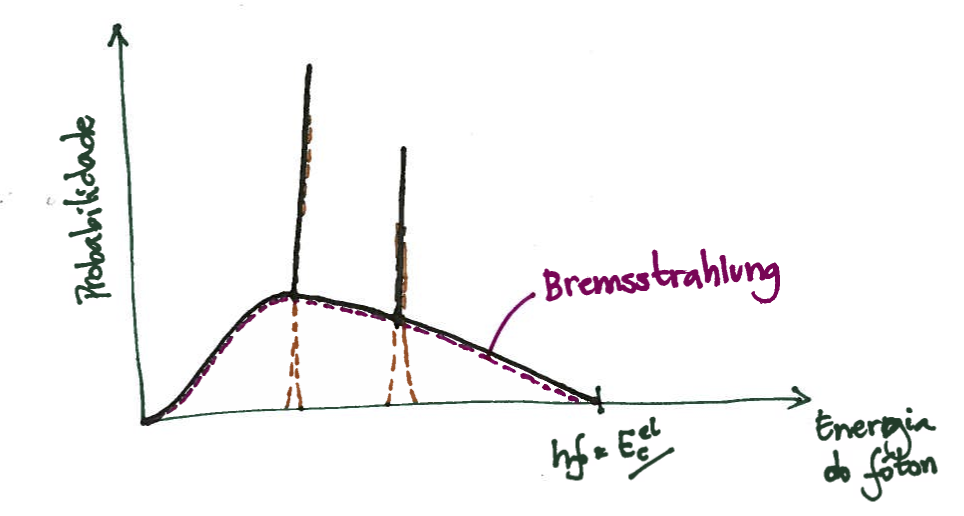
\includegraphics[width=0.9\textwidth]{brem.png}
\caption{\label{fig:brem}Espectro de energia do f\'oton emitido na desacelera\c c\~ao de um el\'etron ao interagir com um material. Note como a distribui\c c\~ao \'e a combina\c c\~ao de dois espectros distintos: um cont\'inuo (em roxo) e um discreto (em laranja). Vejo texto para explica\c c\~ao dos fen\^menos.}
\end{figure}
O espectro de energia dos f\'otons emitidos \'e a superposi\c c\~ao de dois espectros distintos. Um cont\'inuo, que corresponde \`a desacelera\c c\~ao do el\'etron devido \`a intera\c c\~ao com o campo el\'etrico e outro discreto, muito mais intenso mas em energias bem definidas. O espectro cont\'inuo \'e devido ao efeito de Bremsstrahlung descrito nessa se\c c\~ao. Veja na figura como a linha cont\'inua tem um ponto m\'aximo, que corresponde ao caso em que o el\'etron \'e completamente parado e toda sua energia \'e transferida a um \'unico f\'oton.

As linhas de emiss\~ao discretas correspondem a outro tipo de processo at\^omico, que estudaremos em seguida: emiss\~ao e absor\c c\~ao por \'atomos.

\section{Absor\c c\~ao e emiss\~ao de f\'otons por \'atomos}\label{abs}

Quando os \'atomos est\~ao livres, como num g\'as, o espectro de energia dos el\'etrons n\~ao \'e cont\'inuo, como no caso de el\'etrons livre, nem em bandas, como no caso de s\'olidos. As energias que os el\'etrons podem ocupar s\~ao discretas e cada n\'ivel de energia \'e chamado um \textbf{orbital at\^omico}. Calcular a energia de cada um desses orbitais \'e dif\'icil, a n\~ao ser no caso do hidrog\^enio, o que faremos mais a frente.

Como os n\'iveis s\~ao discretos, um el\'etron s\'o vai passar de um n\'ivel para outro se absorver um f\'oton que tem energia dada extamente pela diferen\c ca de energia dos dois orbitais. Esse processo chama\c c\~ao absor\c c\~ao (ou excita\c c\~ao) e \'e esquematicamente represtada por:

\begin{equation}
\text{el\'etron at\^omico ligado} + \text{f\'oton} \rightarrow \text{el\'etron at\^omico ligado}.
\end{equation}
Por conserva\c c\~ao de energia, a freq\"u\^encia de um f\'oton abosrvido entre orbitais com energia $E_1$ e $E_2$ tem que ser:

\begin{equation}
hf + E_1 = E_2.
\end{equation}
Esse processo \'e mostrado na figura \ref{fig:atom}. Em geral, escolhe-se a refer\^encia de energia para el\'etrons at\^omicos como a menor energia que el\'etrons livres podem ter. Essa refer\^encia \'e, como sempre arbitr\'aria (\'e equivalente a dizer qual \'e a ``altitude zero'', tanto faz, \'e apenas um ponto a partir do qual se mede), mas \'e conveniente j\'a que, desta forma, todo el\'etron livre ter\'a energia positiva e todo el\'etron ligado ao \'atomo num orbital ter\'a energia negativa. O processo de absor\c c\~ao \'e representado pela seta marrom apontando para cima. Um el\'etron, num n\'ivel de energia baixo $E_1$, aborve um f\'oton e faz uma transi\c c\~ao para um n\'ivel mais alto $E_2$. Isso s\'o ocorre se a energia do f\'oton for exatamente $E_2-E_1$.

\begin{figure}[ht]
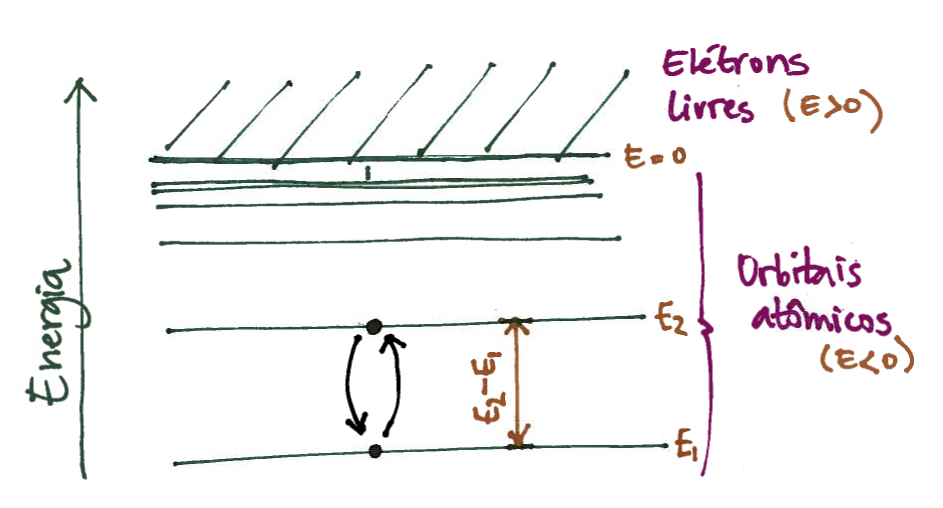
\includegraphics[width=0.9\textwidth]{atom.png}
\caption{\label{fig:atom}N\'iveis de energia de um el\'etron at\^omico. Os estados ligados possuem energia negativa ($E<0$) e existem apenas em n\'iveis de energia discretas. Os el\'etrons livre podem ter qualquer energia positiva $E>0$. Existem infinitos orbitais at\^omicos e a diferen\c ca de energia fica cada vez menor conforme os orbitais se aproximam de zero.}
\end{figure}

Um el\'etron num n\'ivel excitado, depois de um certo tempo, voltar\'a para o estado de menor energia, que \'e o \'unico est\'avel num \'atomo. Esse processo chama-se \textbf{emiss\~ao espont\^anea} e \'e esquematicamente dada pela seguinte rea\c c\~ao:


\begin{equation}
\text{el\'etron at\^omico ligado} \rightarrow \text{el\'etron at\^omico ligado} + \text{f\'oton}.
\end{equation}
Novamente usando conserva\c c\~ao de energia, podemos concluir que a energia do f\'oton ser\'a exatamente a diferen\c ca de energia entre os orbitais:

\begin{equation}
E_2 = E_1 + hf.
\end{equation}
A absor\c c\~ao e emiss\~ao espont\^anea s\~ao os processos pelos quais um \'atomo reage a incid\^encia de luz. Quando um f\'oton incide sobre um \'atomo, se ele tiver a energia correta para induzir uma transi\c c\~ao at\^omica, ele vai ser absorvido e, depois de um certo tempo, reemitido com a mesma frequ\^encia. Esse tempo que demora para ele ser reemitido \'e exatamente o que faz com que a luz, ao passar por um meio com \'atomos pare\c a mais lenta, apesar de cada f\'oton, individualmente, se propagar com a velocidade da luz $c$.

Existe um outro processo pelo qual um el\'etron pode ir de um n\'ivel de maior energia para um n\'ivel de menor energia, chamado de \textbf{emiss\~ao induzida}. Ele \'e esquematicamente dado por:

\begin{equation}
\text{el\'etron at\^omico ligado} + \text{f\'oton} \rightarrow \text{el\'etron at\^omico ligado} + 2\,\text{f\'otons}.
\end{equation}
Esse processo tamb\'em existe que a energia do f\'oton seja igual a diferen\c ca de energia dos orbitais at\^omicos envolvidos na transi\c c\~ao. Al\'em disso, os dois f\'otons no estado final ter\~ao a mesma frequ\^encia e mesma fase, isto \'e, o campo el\'etrico dos dois f\'otons oscilam exatamente da mesma forma (n\~ao necessariamente na mesma dire\c c\~ao, mas com mesma deped\^encia temporal).

Por fim, uma \'ultima possibilidade de intera\c c\~ao de f\'otons com \'atomos \'e o processo de \textbf{ioniza\c c\~ao}. Ele \'e esquematicamente dado por:
\begin{equation}
\text{el\'etron at\^omico ligado} + \text{f\'oton} \rightarrow \text{el\'etron livre}
\end{equation}
Como a energia de el\'etrons livres \'e continua, esse processo n\~ao exige que a energia do f\'oton seja exatamente igual a energia do orbital. Nesse caso, a energia do orbital \'e apenas a energi m\'inima para que o el\'etron se liberte. Qualquer energia acima disso tamb\'em ioniza o \'atomo e o excesso de energia se torna energia cin\'etica para o el\'etron.

\subsection{O \'atomo de hidrog\^enio}\label{sec:hyd}

O \'atomo de hidrog\^enio \'e o mais simples de todos os \'atomos pois possui apenas 1 (um) el\'etron. Nesse caso, os n\'iveis de energia podem ser calculados exatamente. Cada orbital do hidrg\^enio \'e classificado por um n\'umero natural $n\in \mathbb{N}$ e a energia desse n\'ivel \'e dada por:

\begin{equation}\label{eq:ryd}
E_n = -\frac{\text{Ry}}{n^2},
\end{equation}
onde $\text{Ry}$ \'e chamada cosntante de Rydberg e tem valor de $\text{Ry}=13.6\,\text{eV}$. Isso quer dizer que o n\'ivel de menor energia do \'atomo de hidrog\^enio \'e, para $n=1$, $-13.6\,\text{eV}$. Da\'i tamb\'em podemos concluir que qualquer f\'oton com mais de $-13.6\,\text{eV}$ \'e capaz de ionizar o hidrog\^enio. Um f\'oton de $13.6\,\text{eV}$ tem um comprimento de onda de $91\,\text{nm}$, ou seja, hidrog\^enio at\^omico \'e opaco para qualquer comprimento de onda menor que esse. A constante de Rydberg pode ser relacionada com constantes fundamentais da f\'isica da seguinte forma:

\begin{equation}
\text{Ry} = \frac{m_ee^4}{8\epsilon_0h^2},
\end{equation}
onde $m_e$ e $e$ s\~ao, respectivamente, a massa e carga do el\'etron, $\epsilon_0$ \'e a permissividade do v\'acuo e $h$ \'e a constante de Planck.

\subsection{\'Atomos de muitos el\'etrons e degeneresc\^encia dos orbitais}\label{sec:many}

\'Atomos com mais de um el\'etron possuem espectro muito mais complicado que o \'atomo de hidrog\^enio. N\~ao existem rela\c c\~oes simples como \eqref{eq:ryd} para os n\'iveis de energia e os orbitais podem ser calculados apenas aproximadamente. Alguns \'atomos, contudo, tem o espectro eletr\^onico (isto \'e, os n\'iveis de energias dos orbitais em que os el\'etrons podem estar) bem parecidos com o hidrog\^enio e podemos usar os orbitais do hidrog\^enio pelo menos para termos uma id\'eia qualitativa da disposi\c c\~ao dos el\'etrons nos \'atomos.

Uma propriedade importante dos el\'etrons, chamade de \textbf{estat\'istica de Fermi-Dirac}, diz que cada el\'etron num \'atomo tem que estar num orbital diferente. Pode acontecer de diversos orbitais compartilharem o mesmo n\'ivel de energia e, neste caso, dizemos que h\'a um \textbf{degeneresc\^encia}. No \'atomo de hidrog\^enio, cada n\'ivel de energia $n$ possui $2n^2$ orbitais degenerados. Isso quer dizer que, se usarmos um espectro do \'atomo de hidrog\^enio para classificar o estados de um \'atomo com muitos \'eletrons, haver\'a dois el\'etrons ($n=1\Rightarrow 2n^2= 2$) no menor n\'ivel de energia, oito el\'etrons ($n=2\Rightarrow 2n^2=8$) no segundo n\'ivel de energia e por assim adiante. Vale dizer que a maioria dos \'atomos n\~ao s\~ao parecidos com o hidrog\^enio, e essa contagem falha desastrosamente.

Mas o conceito continua importante. Em geral, classificamos os $2n^2$ estados degenerados com o valor do seu momento angular, o valor da proje\c c\~ao do momento angular num eixo arbitr\'ario, e o spin do el\'etron. Esses valores, tal como a energia, tamb\'em s\~ao discretos e representados pelas letras $\ell$, $m$ e $s$ respectivamente. Um n\'ivel de energia $n$ tem $0  \leq \ell \leq n-1$ e $-l \leq m \leq l$. O valor de $s$ \'e sempre $+1/2$ ou $-1/2$. Os diversos valores do momento angular $l$ podem ser representados por $2\ell +1$ caixas, representandos os valores de $m$, como mostra a figura~\ref{fig:manyelectrons}. Dentro de cada caixa, colocamos uma seta para cima e uma para baixo representando os dois valores de spin poss\'iveis para cada el\'etrons. Mais especificamente, a figura~\ref{fig:manyelectrons} mostra a disposi\c c\~ao de um orbital $n=2$ de um \'atomo onde h\'a apenas sete el\'etrons. Ainda caberia mais um el\'etron com essa mesma energia nesse \'atomo.

\begin{figure}[ht]
\begin{center}
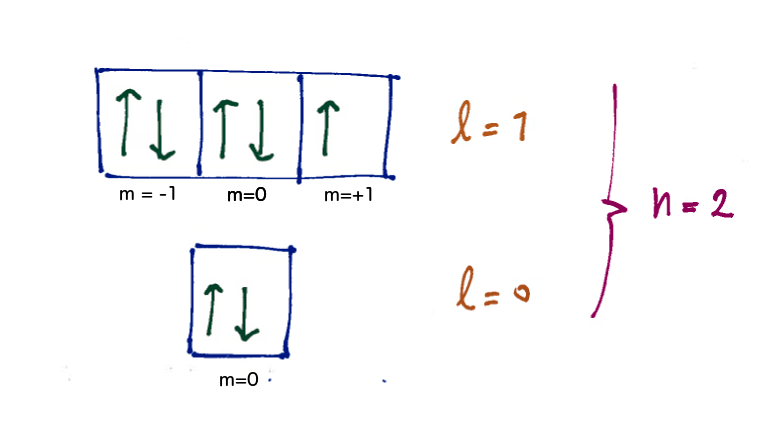
\includegraphics[width=0.8\textwidth]{orbital.png}
\caption{\label{fig:manyelectrons}Exemplo de todos os orbitais degeneradoros do n\'ivel de energia $n=2$ de um \'atomo. Nesse exemplo, o n\'ivel de energia ainda n\~ao est\'a completo, pois ainda caberia um \'ultimo el\'etron no n\'ivel $\ell=2$, $m=+1$ e $s=1/2$.}
\end{center}
\end{figure}


\subsection{O processo de laser}

Como aplica\c c\~ao de todos os processos at\^omicos vistos at\'e agora, vamos estudar como o laser function. Criar f\'otons \'e f\'acil. Criar f\'otons que tenham todos extamente a mesma frequ\^encia e mesma fase, \'e muito mais dif\'icil. Como vimos acima~\ref{abs}, um dos processos pelo qual isso \'e poss\'ivel \'e a emiss\~ao induzida. Nesse processo, se emite um f\'oton sobre um \'atomo excitado. Esse f\'oton tem que ter a mesma energia que uma transi\c c\~ao do el\'etron para o n\'ivel de menor energia. \'E um processo anti-intuitivo, porque em geral se cede energia a um el\'etron para ele ir para um n\'ivel de maior energia. No caso da emiss\~ao induzida, o el\'etron absorve o f\'oton, vai para o n\'ivel de menor energia e emite dois f\'otons com mesma frequ\^encia e mesma fase.

At\'e aqui, nada novo, estou apenas repetindo o que j\'a estudamos acima. A dificuldade desse processo \'e que n\~ao se encontra \'atomos excitados facilmente. Isso porque, el\'etrons em n\'ivel excitados tendem a decair naturalmente para o n\'ivel de menor energia atrav\'es de emiss\~ao espont\^anea. Ent\~ao, a primeira coisa que temos que fazer \'e preparar \'atomos excitados. Para isso, se escolhe \'atomos cujo espectro de energia tenha uma propriedade muito especial: temos que ter tr\^es n\'iveis. A transi\c c\~ao do n\'ivel mais energ\'etico para o n\'ivel intermidário tem que ser r\'apida, enquanto a transi\c c\~ao do n\'ivel intermedi\'ario para o mais baixo tem que ser bem lenta. Isso \'e o que a figura~\ref{fig:laser} mostra.

\begin{figure}[ht]
\begin{center}
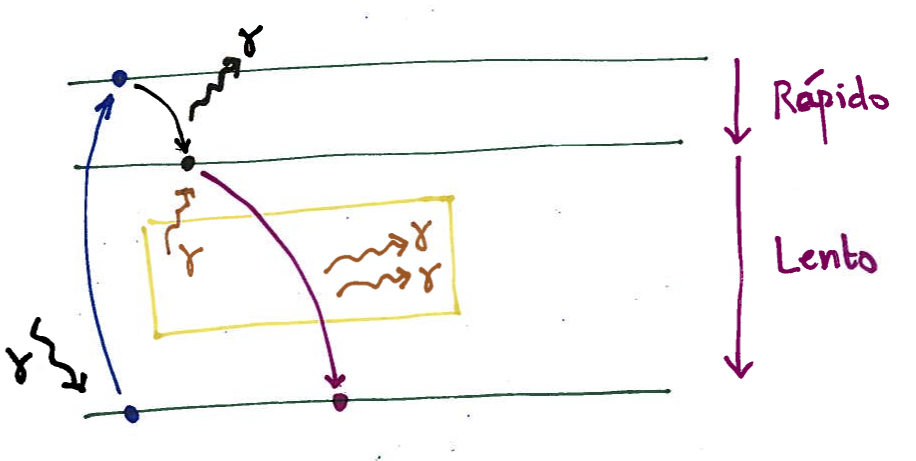
\includegraphics[width=\textwidth]{laser.png}
\caption{\label{fig:laser}Diagrama de n\'iveis de energia mostrando o processo de invers\~ao de popula\c c\~ao e emiss\~ao induzida num laser.}
\end{center}
\end{figure}
Os el\'etrons do \textbf{meio de ganho} do laser come\c cam no n\'ivel de menor energia. Por absor\c c\~ao de f\'otons, a primeira transi\c c\~ao ocorre para o n\'ivel de maior energia (seta azul). Esses el\'etrons decaem por emiss\~ao espont\^anea (seta marrom) rapidamente para o n\'ivel intermedi\'ario, sendo l\'a acumulados. Como a pr\'oxima transi\c c\~ao \'e muito lenta, esse n\'ivel intermedi\'ario serve como um n\'ivel de armazenemanto. Em geral, coloca-se tantos el\'etrons nesse n\'ivel quanto poss\'ivel (isto \'e, at\'e o limite de degeneresc\^encia do n\'ivel de energia, como visto em~\ref{sec:many}). Quando o n\'ivel intermedi\'ario est\'a cheio, diz-se que a \textbf{popula\c c\~ao est\'a invertida}.

O segundo passo \'e jogar um f\'oton com a energia exata de transi\c c\~ao entre o n\'ivel intermedi\'ario e o mais baixo. Os el\'etrons v\~ao absorver esse f\'oton, fazer a transi\c c\~ao para o n\'ivel mais baixo e emitir dois f\'otons com a mesma frequ\^encia (emiss\~ao induzida, seta roxa). Em lasers reais, se coloca esses \'atomos entre dois espelhos de forma que os f\'otons emitidos voltem, atingem mais el\'etrons no n\'ivel intermedi\'ario e se multipliquem ainda mais.

Esse processo de multiplica\c c\~ao de f\'otons com mesma frequ\^encia e fase (como na caixa amarela) \'e o que se chama de \textbf{laser}.

\section{As fun\c c\~oes de onda de De Broglie}

\epigraph{Nous devons donc envisager l'\'etat présent de l'universe comme l'effet de son \'etat ant\'erieur, et comme la cause de celui qui va suivre. Une intelligence qui pour un instant donn\'e conna\^itrait toutes les forces dont la nature est anim\'ee et la situation respective des \^etres qui la composent, si d'ailleurs elle \'etait assez vaste pour soumettre ces donn\'ees \`a l'analyse, embrasserait dans la m\^eme formule les mouvements des plus grands corps de l'universe et ceux du plus l\'eger atome; rien ne serait incertain pour elle, et l'avenir comme le passé serait présent a ses yeux.}{Pierre-Simon Laplace}

Apesar de ser claro que radia\c c\~ao eletromagn\'etica \'e um fen\^omeno ondulat\'orio, pois podemos observar efeitos como interfer\^encia e difra\c c\~ao, at\'e esse momento temos pensado na luz como se fosse uma part\'icula hipot\'etica chamada f\'oton. Essa part\'icula, contudo, ainda possui as mesma propriedades de um fen\^omeno ondulat\'orio como frequ\^encia e comprimento de onda. Essa ``dualidade'' existe pois estamos tentando usar conceitos cl\'assicos, como uma onda eletromagn\'etica ou uma part\'icula pontual, para descrever efeitos que s\~ao essencialmente qu\^anticos.

A realidade \'e que a mec\^anica qu\^antica n\~ao pode ser descrita por nenhum desses dois objetos individualmente, mas atrav\'es de algo que se chama \textbf{fun\c c\~ao de onda}. A fun\c c\~ao de onda \'e o objeto fundamental da mec\^anica qu\^antica da mesma forma que uma part\'icula pontual \'e o objeto fundamental da mec\^anica cl\'assica. Na mec\^anica cl\'assica, podemos imaginar que todo e qualquer objeto como uma superposi\c c\~ao de part\'iculas pontuais e, se descrevermos a din\^amica de uma part\'icula pontual, o que \'e feito na segunda lei de Newton, ent\~ao podemos descrever a din\^amica de qualquer corpo material. Na mecânica qu\^antica o objeto fundamental \'e a fun\c c\~ao de onda do sistema. Todo e qualquer sistema na mec\^anica qu\^antica \'e descrito por uma fun\c c\~ao $\psi(x,t)$ que, para cara instante de tempo $t$, associa um valor a cada ponto do espa\c co $x$. A evolu\c c\~ao temporal dessa fun\c c\~ao \'e descrita pela equa\c c\~ao de Schr\"odinger, mas isso \'e fora do escopo desse resumo.

A chamada ``interpreta\c c\~ao de Conpehagen'' da fun\c c\~ao de onda $\psi(x,t)$, associa o m\'odulo ao quadrado dessa fun\c c\~ao $|\psi(x,t)|^2$ como a probabilidade de medir a part\'icula que ela descreve na posi\c c\~ao $x$. Note que, como a fun\c c\~ao de onda \'e algo que se estende no espa\c co, a medida da posi\c c\~ao de uma part\'icula pode resultar em v\'arios resultados distintos. Em particular, a fun\c c\~ao de onda de uma part\'icula livre com momento $p$ e energia $E$ \'e escrita como:

\begin{equation}
\psi(x,t) = e^{-i(Et - px)}.
\end{equation}
O m\'odulo ao quadrado dessa fun\c c\~ao \'e $|\psi(x)|^2 = 1$, ou seja, constante em todos os pontos do espa\c co. Isto \'e equivalente a dizer que n\~ao podemos dizer onde uma part\'icula qu\^antica est\'a, apesar de sabermos seu momento linear e sua energia. Tal como o ponto material \'e uma idealiza\c c\~ao da mec\^anica cl\'assica, a part\'icula livre tamb\'em \'e uma idealiza\c c\~ao da mec\^anica qu\^antica.

A fun\c c\~ao de onda da part\'icula livre se comporta como uma onda plana. Se separamos a parte real e imagin\'aria da fun\c c\~ao acima teremos:
\begin{equation}
\psi(x,t) = \cos(px - Et) + i\sin(px - Et),
\end{equation}
de onde \'e \'obvio que essa fun\c c\~ao se comporta como uma onda com frequ\^encia $f$ e comprimento de onda $\lambda$ dados por:

\begin{equation}
\begin{split}
&E = hf\\
&p = \frac{h}{\lambda}
\end{split}
\end{equation}
Essas rela\c c\~oes s\~ao exatamente as mesmas que v\'inhamos usando para a energia e momento do f\'oton e s\~ao chamadas de \textbf{rela\c c\~oes de De Broglie}. O pulo conceitual que o De Broglie prop\^os \'e que a fun\c c\~ao de onda de todas as part\'iculas livres obedecem essas mesmas rela\c c\~oes.

\subsection{O experimento de dupla-fenda}

O experimento de dupla fenda \'e uma experi\^encia cl\'assica que demonstra a interfer\^encia de ondas. A id\'eia \'e simples e resumida na figura~\ref{fig:dupla_fenda}.

\begin{figure}[ht]
\begin{center}
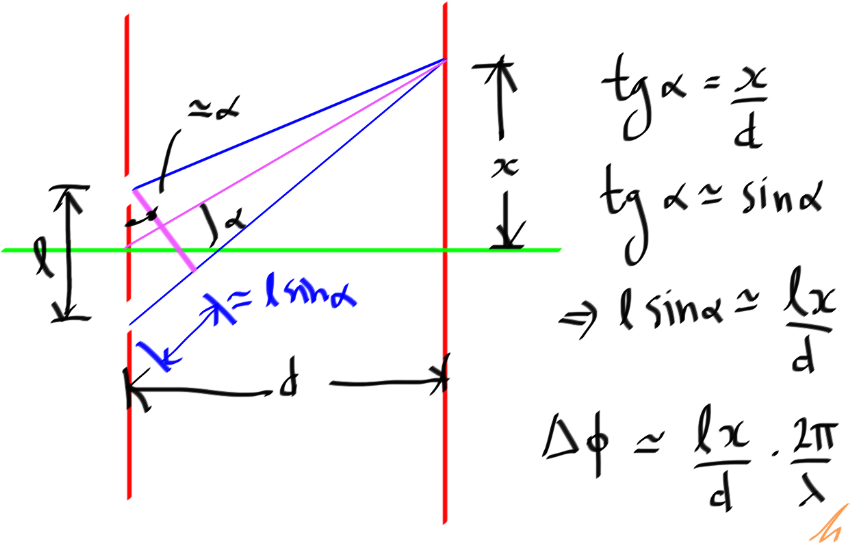
\includegraphics[width=0.7\textwidth]{dupla_fenda.png}
\caption{\label{fig:dupla_fenda} Experimento de dupla fenda de Young. As aproxima\c c\~oes na figura s\~ao v\'alidas para \^angulos $\alpha$ pequenos, isto \'e, para $x$ pequenos.}
\end{center}
\end{figure}

A id\'eia \'e ter uma fonte de luz do lado esquerdo do arranjo experimental. Essa fonte de luz incide sobre o anteparo com duas fentas. Pelo \textbf{princ\'ipio de Huygens}, podemos pensar em cada uma dessas fendas como uma fonte pontual de luz. O caso interessante \'e quando essas duas fontes s\~ao coerentes, isto \'e, quando as fases das ondas emanadas de cada uma das fendas s\~ao iguais.

Nesse caso, a diferen\c ca entre as dist\^ancias percorridas por cada raio de luz que atinge o anteparo mais a direita tamb\'em d\'a a diferen\c ca de fase com que as duas ondas se superp\~oem. Para dist\^ancias n\~ao muito grandes do ponto central entre as duas fendas, podemos fazer a seguinte aproxima\c c\~ao:

\begin{equation}
\sin\alpha \approx \tan\alpha = \frac{x}{d},
\end{equation}
onde a defini\c c\~ao das quantidades est\~ao todas na figura. Tamb\'em podemos aproximar a diferen\c ca entre os caminhos percorridos entre os dois feixes de luz como:

\begin{equation}
l\sin\alpha\approx \frac{\ell x}{d},
\end{equation}
o que resulta numa diferen\c ca de fase de:

\begin{equation}
\Delta\phi = \frac{\ell x}{d}\times\frac{2\pi}{\lambda}.
\end{equation}
Ent\~ao, a uma dada dist\^ancia $x$ do ponto m\'edio entre as fendas, para uma dit\^ancia $d$ entre os aparatos, uma dist\^ancia $\ell$ entre as fendas e um comprimento de onda $\lambda$, temos a seguinte amplitude:

\begin{equation}
\sin(\phi^{\prime}) + \sin(\phi^{\prime} + \Delta\phi) = 2\sin(\phi^{\prime} + \frac{\Delta\phi}{2})\cos(\frac{\Delta\phi}{2}),
\end{equation}
onde $\phi^{\prime}$ \'e uma fase arbitr\'aria. O segundo termo do produto \'e o interessante. Vemos que se $\frac{\Delta\phi}{2} = \frac{\pi}{2}$, a amplitude ser\'a zero. Isso \'e f\'acil de entender, j\'a que uma diferen\c ca de fase de $\pi$ entre as duas ondas d\'a claramente uma interfer\^encia destrutiva. De uma forma geral, a posi\c c\~ao dos m\'inimos de interfer\^encia s\~ao dadas por:

\begin{equation}
\frac{\Delta\phi}{2} = n\pi + \frac{\pi}{2} \Rightarrow \frac{\ell x}{d\lambda} = n + \frac{1}{2}; \qquad n\in\mathbb{Z},
\end{equation}
o primeiro m\'inimo ser\'a quando $n=0$, isto \'e $x = \frac{d\lambda}{2\ell}$.

Essa \'e a experi\^encia cl\'assica de Young. O interessante \'e exatamente a mesma coisa acontece para qualquer tipo de part\'icula, pelas rela\c c\~oes de De Broglie, bastando relacionar o momento linear com o comprimento de onda. Como a fun\c c\~ao de onda obedece o mesmo tipo de rela\c c\~ao, a soma das duas fun\c c\~oes de onda tamb\'em ter\'a pontos em que o valor vai a zero e, logo, pela interpreta\c c\~ao de Conpehagem, s\~ao pontos em que os el\'etrons (ou outra part\'icula qualquer) nunca s\~ao detectados. Usando a rela\c c\~ao de De Broglie, vemos que a posi\c c\~ao da primeira linha no segundo anteparo em que el\'etrons nunca ser\~ao detectados \'e:

\begin{equation}
x = \pm\frac{hd}{2p\ell}
\end{equation}

\subsection{Raio X caracter\'istico e efeito Auger}

Vamos revisitar o espectro de produ\c c\~ao de raio X como visto na figura~\ref{fig:brem}. N\'os vimos que um espectro real\'istico \'e composto de duas partes: uma cont\'inua, devido ao Bremsstrahlung, e alguns picos. Agora podemos entender a origem dos picos. Os el\'etrons, quando s\~ao freiados ao passar por um material, podem n\~ao apenas ser desacelerados, mas tamb\'em fazer um efeito similar ao efeito fotoel\'etrico nos el\'etrons do material. Na pr\'atica, usando as id\'eias de De Broglie, o efeito \'e exatamente o mesmo: se a frequ\^encia associada \`a fun\c c\~ao de onda do el\'etron for tal que \'e capaz de liberar um el\'etron da estrutura do material, quando esse el\'etron se recombinar, ele emitir\'a um f\'oton.

Uma outra possibilidade, que n\~ao discutimos aqui, mas \'e interessante, \'e que a energia de recombina\c c\~ao n\~ao seja usada para emitir f\'otons, mas sim para liberar um segundo el\'etron. Nesse caso, esse el\'etron \'e conhecido como \textbf{el\'etron Auger}.

\section{Decaimentos nucleares}

O processo de decaimento nuclear radioativo \'e um processo aleat\'orio, que acontece independentemente da hist\'oria passada do n\'ucleo e, em primeira aproxima\c c\~ao, da presen\c ca de outros n\'ucleos radioativos. Como o processo \'e aleat\'orio, tudo que podemos dizer \'e a probabilidade de um n\'ucleo decair num dado intervalo de tempo, mas n\~ao \'e poss\'ivel ter certeza se, ap\'os passagem de dado tempo o n\'ucleo ter\'a decaido ou n\~ao. A probabilidade de um n\'ucleo decair num certo intervalo de tempo $\Delta t$ \'e dado por:

\begin{equation}
P(\Delta t) = \lambda\times \Delta t.
\end{equation}
Note como a probabilidade n\~ao depende da hist\'oria anterior do n\'ucleo. N\~ao importa se um n\'ucleo radioativo \'e antigo ou velho, a probabilidade de decair num intervalo de tempo $\Delta t$ s\'o depende do intervalo e de $\lambda$.

Se tivermos uma cole\c c\~ao grande de n\'ucleos radioativos, como a probabilidade de cada n\'ucleo decair independete dos outros, em m\'edia, teremos $N \lambda \Delta t$ n\'ucleo deca\'idos ap\'os um intervalo de tempo $\Delta t$. Uma outra forma de dizer isso \'e que a velocidade de desaparecimento dos n\'ucleos \'e:

\begin{equation}\label{eq:atividade}
\frac{\Delta N}{\Delta t} = -\lambda N,
\end{equation}
onde o signal negativo apenas indica que os n\'ucleos est\~ao desparecendo. A quantidade no lado direito da equ\c c\~ao \eqref{eq:atividade}, $\lambda N$, chama-se \textbf{atividade} da amostra radioativa e indica quantos decaimentos, em m\'edia, se observa por unidade de tempo. Embora n\~ao seja imediato, podemos ``resolver'' a equa\c c\~ao acima para obter uma fun\c c\~ao da quantidade m\'edia de n\'ucleos que ainda se preservam sem decair depois de um tempo $t$:

\begin{equation}\label{eq:decay}
N(t) = N(0)\times e^{-\lambda t}.
\end{equation}
A quantidade $N(0)$ denota quantos n\'ucleos sua amostra tem no in\'icio da observa\c c\~ao, isto \'e, no tempo $t=0$. Como essa rela\c c\~ao envolve a fun\c c\~ao exponencial, uma pequena revis\~ao \'e em ordem.

\subsection{Fun\c c\~oes exponenciais e logar\'itimicas}

A fun\c c\~ao exponencial:
\begin{equation}
\begin{split}
&f:\mathbb{R}\rightarrow \mathbb{R},\\
&f(x) = e^x,
\end{split}
\end{equation}
\'e definida para todos os reais e possui as seguintes propriedades:

\begin{enumerate}
\item $f(x+y)= e^{x+y} = e^x\times e^y = f(x)\times f(y)$,
\item $f(x-y) = e^{x-y}= \frac{e^x}{e^y} = \frac{f(x)}{f(y)}$,
\item $f(xy) = e^{xy} = (e^x)^y = f(x)^y$.
\end{enumerate}

A fun\c c\~ao logar\'itmo

\begin{equation}
\begin{split}
&g:\mathbb{R}^+\rightarrow \mathbb{R},\\
&g(x) = \ln x,
\end{split}
\end{equation}
 \'e definida como a fun\c c\~ao inversa da exponencial, isto \'e:

\begin{equation}
f(x) = e^x \rightarrow g(x) = f^{-1}(x) = \ln x \rightarrow f(g(x)) = x\text{ e }g(f(x)) = x,
\end{equation}
ou, dito de outra forma:

\begin{equation}
y = e^x \leftrightarrow x = \ln y.
\end{equation}
As propriedades da fun\c c\~ao logar\'itimo seguem imediatamente das propriedades da fun\c c\~ao exponencial:

\begin{enumerate}
\item $f(xy) = \ln(xy) = \ln x + \ln y = f(x) + f(y)$,
\item $f(\frac{x}{y}) = \ln\frac{x}{y} = \ln x - \ln y = f(x) - f(y)$,
\item $f(x^y) = \ln x^y = y\ln x = y\, f(x)$.
\end{enumerate}
A propriedade que mais vamos usar aqui nesse texto \'e realmente o fato do logar\'itmo ser o inverso da exponencial:

\begin{equation}
\begin{split}
&e^{\ln x} = x\\
&\ln (e^x) = x
\end{split}
\end{equation}

\subsection{Meia-vida e vida m\'edia}

A \textbf{meia-vida}, $t_{1/2}$, de uma amostra \'e definida com o tempo em que, em m\'edia, apenas metade da amostra sobrevive. Usando a equ\c c\~ao \eqref{eq:decay}:
\begin{equation}
N(t_{1/2}) = \frac{N(0)}{2} = N(0) e^{-\lambda t_{1/2}}.
\end{equation}
Dividindo por $N(0)$ dos dois lados e tirando o logar\'itmo:

\begin{equation}
\ln\frac{1}{2} = -\lambda t_{1/2} \Rightarrow t_{1/2} = \frac{\ln(2)}{\lambda},
\end{equation}
onde usamos que $-\ln\frac{1}{2} = \ln 2$, o que pode ser observado sem maiores dificuldades das propriedades do logar\'itmo sabendo que $\ln(1) = 0$.

A \textbf{vida m\'edia}, $\tau$, de um n\'ucleo \'e o tempo que, em m\'edia, que demora para ele decair. Novamente, essa conta n\~ao \'e imediata mas \'e poss\'ivel mostrar que esse tempo \'e dado por:
\begin{equation}
\tau = \frac{1}{\lambda}
\end{equation}

\subsection{Tipo de decaimentos radioativos}

Um n\'ucleo \'e composto de pr\'otons e n\^eutrons. Da mesma forma que os el\'etrons num \'atomo ocupam orbitais de energia em n\'iveis discretos, os pr\'otons e n\^eutrons tamb\'em apenas existem em n\'iveis de energia bem definidos. Ainda da mesma forma que el\'etrons num \'atomo (reveja a se\c c\~ao~\ref{abs} se voc\^e n\~ao se recorda), esses pr\'otons e n\^eutrons podem estar num n\'ivel de energia que n\~ao \'e aquele com menor energia poss\'ivel. E, mais uma vez da mesma forma que el\'etrons num \'atomo, esses pr\'otons e n\^eutrons, dado um tempo sufienciente, v\~ao voltar ao n\'ivel de menor energia, pois esse \'e o \'unico est\'avel, emitindo um f\'oton (em geral em frequ\^encias bem maior que a luz vi\'isivel, j\'a que as energias das liga\c c\~oes at\^omicas s\~ao bem maiores que as dos el\'etrons num \'atomos). Esse tipo de decaimento que acontece com n\'ucleos excitados chama-se \textbf{decaimento gama}.

\begin{equation}
\text{n\'ucleo excitado} \rightarrow \text{n\'ucleo desexcitado} + \text{f\'oton}.
\end{equation}

Uma outra possibilidade \'e que pr\'otons e n\^eutrons decaiam atrav\'es da chamada for\c ca nuclear fraca. Nesse caso, o processo n\~ao emite f\'otons, mas uma part\'icula chamada b\'oson $W$. O b\'oson $W$, por sua vez, decai quase que imediatamente em um el\'etron ou p\'ositron, da seguinte forma:

\begin{equation}\label{beta}
\begin{split}
&n \rightarrow p + W^-\rightarrow p + e^- + \bar{\nu},\\
&p \rightarrow n + W^+\rightarrow p + e^+ + \nu,
\end{split}
\end{equation}
onde $e^+$ representa um p\'ositron, $e^-$ um el\'etron e $\nu$ s\~ao neutrinos. Na equa\c c\~ao~\eqref{beta}, o primeiro processo chama-se \textbf{decaimento $\beta -$} e o segundo \textbf{decaimento $\beta +$}. Como a massa do n\^eutron \'e essecialmente a mesma da do pr\'oton, a massa do n\'ucleo n\~ao muda, mas sim o n\'umero at\^omico. No final do dia, o efeito de um decaimento beta para o n\'ucleo \'e, respectivamente para $\beta -$ e $\beta +$:

\begin{equation}
\begin{split}
&{}^Z_AN \rightarrow {}^{Z+1}_AN + e^- + \bar{\nu},\\
&{}^Z_AN \rightarrow {}^{Z-1}_AN + e^+ + \nu.
\end{split}
\end{equation}

Finalmente, o n\'ucleo pode simplesmente se quebrar emitindo parte da sua estrutura. Os casos mais comuns s\~ao a emiss\~ao de um n\'ucleo de h\'elio, o que \'e chamado de \textbf{decaimento alfa}:

\begin{equation}
{}^Z_AN \rightarrow {}^{Z-2}_{A-4}N + {}^2_4\alpha,
\end{equation}
a emiss\~ao de n\^eutron (que n\~ao tem nenhum nome em particular):

\begin{equation}
{}^Z_AN \rightarrow {}^{Z}_{A-1}N + {}^0_1n,
\end{equation}
ou a quebra em dois n\'ucleos pesados:

\begin{equation}
{}^Z_AN \rightarrow {}^{Z_1}_{A_1}N_1 + {}^{Z_2}_{A_2}N_2,
\end{equation}
tal que $Z = Z_1 + Z_2$ e $A = A_1 + A_2$ e esse processo \'e chamado, genericamente, de \textbf{fiss\~ao nuclear}.

Todos esses processos obedecem a mesma lei de decaimento mas, claro, se um mesmo n\'ucleo decair de duas formas diferentes, os processos ter\~ao constantes de decaimento diferentes.

\subsection{Um adendo sobre unidades}

Por raz\~oes hist\'oricas, as unidades para as grandezas relacionadas \`a decaimentos radioativos s\~ao uma confus\~ao. Aqui eu vou tentar sistematizar aquelas que s\~ao mais encontradas.

\begin{description}
\item[Dose absorvida] A dose absorvida diz d\'a a quantidade de energia proveniente de produtos de decaimento radioativo que um corpo absorve por unidade de massa. A unidade no SI \'e o $\text{Gray (Gy)} = 1\,\text{J/kg}$. Contudo, a unidade mais comum \'e o $\text{rad} = 100\,\text{erg/g} = 0.01\,\text{Gy}$.
\item[Atividade] Como j\'a visto, a atividade de uma fonte radioativa diz quantos decaimentos h\'a por unidade de tempo. A unidade no SI \'e o $\text{Bequerel (Bq)} = 1/\text{s}$. A unidade mais comum, contudo, \'e o $\text{Curie (c)} = 3.7\times 10^{10}\,\text{Bq}$.
\item[Flu\^encia] A flu\^encia diz quanto de \'area foi exposta a radia\c c\~ao. Ou seja, quantas part\'iculas provenientes de decaimentos radioativos foram absorvidas por \'area. A unidade no SI \'e o $1/\text{m}^2$, mas a unidade mais usada \'e o $1/\text{cm}^{2}$.
\item[Dose equivalente] Os efeitos biol\'ogicos de uma radia\c c\~ao depende de diversos fatores: que tipo de part\'icula foi absorvida ($\alpha$, $\beta$, $\gamma$, n\^eutrons, $\ldots$), em que parte do corpo a energia foi absorvida (\'org\~aos vitais n\~ao, \'org\~ao com r\'apida reprodu\c c\~ao celular ou n\~ao, $\ldots$), qu\~ao r\'apida foi a absor\c c\~ao (doses agudas ou n\~ao) e muitos outros fatores que s\~ao dif\'iceis de listar aqui e mesmo de se avaliar. O pessoal que regulamenta a atividade de prote\c c\~ao contra radia\c c\~ao cria um n\'umero, chamado RBE (relative biological effect) que diz o quanto uma radia\c c\~ao \'e perigosa. Quanto maior esse n\'umero, maior o impacto biol\'ogico que a radi\c c\~ao. Esse n\'umero \'e multiplicado pela dose absorvida para dar a \textbf{dose equivalente}. Se o RBE for multiplicado pela dose em Gray, a unidade resultante \'e o Sievert (Sv), enquanto se o RBE for multiplicado pela dose em rad, a unidade resultante \'e o rem, que \'e de longe a quantidade mais usada quando o assunto \'e efeitos biol\'ogicos da radioatividade.
\end{description}

\subsection{Energia de liga\c c\~ao e d\'eficit de massa}

\epigraph{Our Sun is a second- or third-generation star. All of the rocky and metallic material we stand on, the iron in our blood, the calcium in our teeth, the carbon in our genes were produced billions of years ago in the interior of a red giant star. We are made of star-stuff.}{Carl Sagan}

A massa de um n\'ucleo \'e menor que a soma das massas dos seus constituintes. Vamos supor nessa discuss\~ao que o n\'ucleo tenha $n_p$ pr\'otons e $n_n$ n\^eutrons. Isso quer dizer que:

\begin{equation}
m_{N} < n_pm_p + n_nm_n,
\end{equation}
onde $m_p$ \'e a massa do pr\'oton e $m_n$ \'e a massa do n\^eutron (elas s\~ao bem parecidas, mas n\~ao importa para essa discuss\~ao). A energia de um corpo livre em repouso \'e dada por:

\begin{equation}
E = mc^2.
\end{equation}
Ent\~ao isso quer dizer que a energia do n\'ucleo $m_Nc^2$ \'e menor que a energia que voc\^e teria se voc\^e tivesse separado todos os pr\'otons e n\^eutrons que o formam. A diferen\c ca de energia

\begin{equation}
\Delta E_N = m_{N}c^2 - (n_pm_p + n_nm_n)c^2
\end{equation}
\'e interpretada como a energia que mant\'em os pr\'otons e n\^eutrons ligados. Essa energia \'e negativa, como \'e o caso tamb\'em no el\'etron no \'atomo de hidrog\^enio que vimos na se\c c\~ao~\ref{sec:hyd}.

Uma consequ\^encia interessante dessa rela\c c\~ao \'e estudar a energia de liga\c c\~ao por constituinte para diferentes n\'ucleos. A id\'eia \'e a seguinte: para todos os n\'ucleos a massa \'e menor que a massa dos constituintes. Mas e se n\~ao separ\'assemos todos os constituintes, mas apenas quebr\'assemos o n\'ucleo em dois outros n\'ucleos, menores, mas ainda compostos de v\'arios pr\'otons e n\^eutrons? A massa de cada um deles ainda \'e menor que a massa de cada um dos seus constituintes, mas a massa dos dois n\'ucleos menores pode ser maior ou menor que a massa do n\'ucleo maior (a rela\c c\~ao n\~ao \'e linear, por isso que h\'a esse efeito). A figura~\ref{fig:bind_ener} mostra a quantidade:

\begin{equation}
-\frac{\Delta E_N}{n_p+n_n},
\end{equation}
para diversos n\'ucleos em fun\c c\~ao do n\'umero de massa $A=n_p+n_n$.

\begin{figure}[ht]
\begin{center}
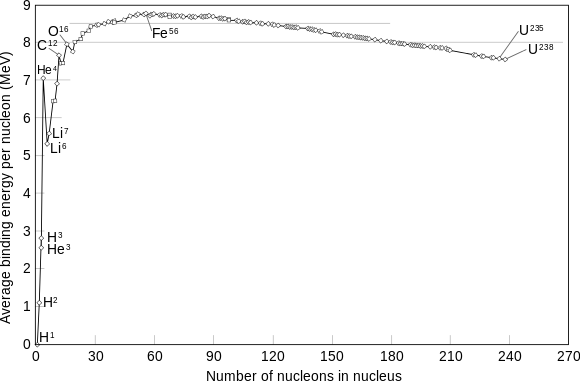
\includegraphics[width=0.7\textwidth]{binding_energy.png}
\caption{\label{fig:bind_ener}A energia m\'edia de liga\c c\~ao por consitutinte dos n\'ucleos at\^omicos. Note como o ferro ($A=56$) \'e o n\'ucleo mais est\'avel pois tem a maior energia (em valor absoluto) por constituinte (gr\'afico copiada da Wikipedia).}
\end{center}
\end{figure}
Atrav\'es desse gr\'afico, podemos estudar o que acontece com a energia total no processo

\begin{equation}\label{fisfus}
{}_AN \leftrightarrow {}_{A_1}N_1 + {}_{A_2}N_2,
\end{equation}
tal que $A = A_1 + A_2$, ou seja, um processo de fiss\~ao (esquerda para direita) ou fus\~ao nuclear (direita para esquerda). Pelo gr\'afico pode-se ver que, se todos os n\'ucleos envolvidos estiverem antes do ferro ($A=56$), a energia de $N$ ser\'a menor (lembre-se que o gr\'afico \'e de menos a quantidade $\Delta E$) que a energia de $N_1$ e $N_2$ separadamente. Isto \'e, o n\'ucleo grande \'e mais est\'avel. Outra forma de dizer isso \'e que, para elementos leves at\'e o ferro o processo espont\^aneo \'e a fus\~ao nuclear.

J\'a no caso em que os n\'ucleos mais pesados que o ferro, a energia do n\'ucleo $N$ \'e maior que a soma das energias dos n\'ucleos $N_1$ e $N_2$. \'E por isso que n\'ucleos muito pesados, como o ur\^anio e o pol\^onio sofrem fiss\~ao nuclear espont\^anea. Mais do que isso, num ambiente energ\'etico o suficiente para que essas rea\c c\~oes possam acontecer, o equil\'ibrio da equa\c c\~ao~\eqref{fisfus} tende para esquerda em n\'ucleos leves e para direita em n\'ucleos pesados. Ent\~ao, por exemplo, no in\'icio do universo, quando ele era muito quente, elementos at\'e o ferro puderam se formar espontaneamente. Mas elementos mais pesados que o ferro, mesmo que se formassem eventualmente, eram mais prov\'aveis que desaparecerem espontaneamente do que restarem para formar estruturas no universo.

Os elementos pesados, que s\~ao t\~ao importantes para a vida na Terra, n\~ao v\^em de rea\c c\~oes espont\^aneas entre n\'ucleos, mas sim de colis\~oes de alt\'issimas energias entre n\'ucleos no interior das estrelas, onde a press\~ao \'e t\~ao grande que for\c ca a produ\c c\~ao desses n\'ucleos pesados. E \'e por isso que, de certa forma, somos todos poeira de estrela.

\subsection{Data\c c\~ao por ${}^{14}C$}

Existem tr\^es is\'otopos de carbono na natureza: dois est\'aveis: ${}^{12}C$ e ${}^{13}C$, e um que sofre decaimento $\beta$: ${}^{14}C$. O ${}^{14}C$ \'e produzido por raios c\'osmicos que incidem na atmosfera terrestre. Como a taxa de incid\^encia de raios c\'osmicos \'e mais ou menos constante, bem como o decaimento do ${}^{14}C$ por decaimento $\beta$, ent\~ao a propor\c c\~ao de ${}^{14}C$ na atmosfera \'e mais ou menos constante. Como os ciclo do carbono nos vegetais n\~ao distingue entre os is\'otopos, essa propor\c c\~ao \'e mais ou menos a mesma que \'e encontrada em vegetais. E como os vegetais s\~ao a base de toda cadeia alimentar, a propor\c c\~ao de carbono \'e mais ou menos a mesma em todas as coisas vivas.

A meia-vida do ${}^{14}C$ \'e de 5730 anos, o que \'e bem adequada para data\c c\~ao hist\'orica. Assim, medindo a atividade $\beta$ proveniente de uma amostra de material, podemos escrever:

\begin{equation}
\frac{N}{N_0}
\end{equation}

\end{document}

